\section{Résultats supplémentaires}
\label{sec:resultats_bonus}

\begin{table}[h]
    \centering
    \begin{tabulary}{\linewidth}{c c c c}
        \toprule
         & Cuivre & Aluminium & Acier \\
        \midrule
        Echantillon 1 & \(4 \pm 0.25\) \si{\milli\meter} & \(6 \pm 0.25\) \si{\milli\meter} & \(6 \pm 0.25\) \si{\milli\meter}\\
        Echantillon 2 & \(2.5 \pm 0.25\) \si{\milli\meter} & \(5 \pm 0.25\) \si{\milli\meter} & \(6 \pm 0.25\) \si{\milli\meter} \\
        \bottomrule
    \end{tabulary}
    \caption{Épaisseurs des échantillons testés sur le transformateur PHYWE}
    \label{tab:thiccness}
\end{table}

TODO: citer la figure en dessous qqpart
\begin{figure}[h]
    \begin{minipage}{0.48\linewidth}
        \centering
        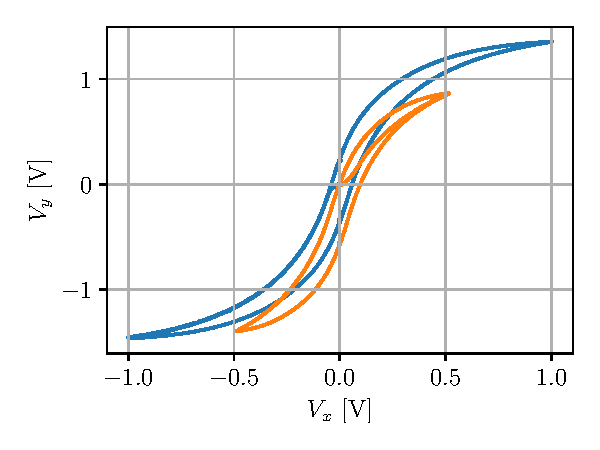
\includegraphics[width=\linewidth]{figures/phywe_autres_cycles.pdf}
        \caption{Différents cycles d'hystérèse du bloc PHYWE}
        \label{fig:autres_cycles}
    \end{minipage}
    \hfill
    \begin{minipage}{0.48\linewidth}
        \centering
        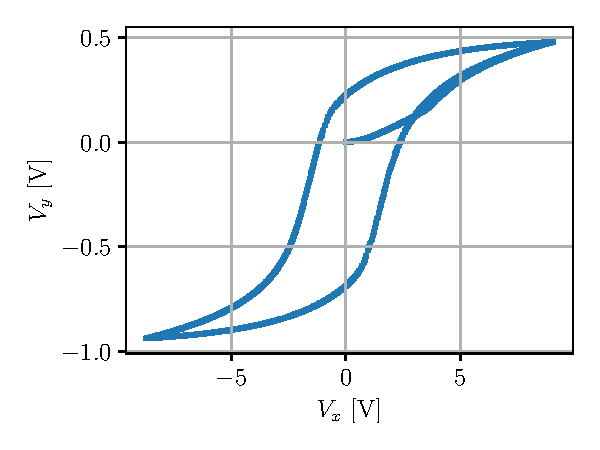
\includegraphics[width=\linewidth]{figures/G1-anneau.pdf}
        \caption{Hystérèse du transformateur en anneau}
        \label{fig:anneau}
    \end{minipage}
\end{figure}

\section{Calcul d'erreurs}
\label{sec:erreurs}

Les erreurs sur les mesures sont données dans le \autoref{tab:erreurs}.

\begin{table}[h]
    \centering
    \begin{tabulary}{\textwidth}{C C C}
        \toprule
        Variable & Erreur & Commentaire \\
        \midrule
        \(V_x\) [\si{\volt}] & 0.0001 & Basé sur les chiffres significatifs de la mesure \\
        \(V_y\) [\si{\volt}] & 0.0001 & Basé sur les chiffres significatifs de la mesure \\
        \(R\) [\si{\ohm}] & 0.01 & Indiqué sur la resistance \\
        \(N\) & 0 & Nombre de spires supposé exact \\
        \bottomrule
    \end{tabulary}
    \caption{Erreurs estimées sur les mesures}
    \label{tab:erreurs}
\end{table}

\paragraph*{Regression linéaire}
Les erreurs sur les fits linéaires \(y = ax + b\) sur les mesures \((x_i, y_i) ; i = \{1, \hdots, n\}\) sont donnés par l'équation \cite{erreursmesure}:

\begin{equation}
    \label{eq:erreur:fit}
    \begin{aligned}
        (\Delta a)^2 &= \frac{\sum_{i=1}^{n}(y_i - (a x_i + b))^2}{(n-2) \sum_{i=1}^{n}(x_i - \bar{x})^2}\\
        \Delta b &= \bar{x} \Delta a + a \Delta \bar{x}
    \end{aligned}
\end{equation}

En pratique, ces valeurs sont calculées par la bilbiothèque python \texttt{numpy}.

\paragraph*{Formules d'erreurs}
L'erreur sur la pente moyenne \(\bar{\beta}\) du domaine linéaire est donnée par

\begin{equation}
    \Delta \bar{\beta} = \left|\Delta \beta_1\right| + \left|\Delta \beta_2\right|
\end{equation}

L'erreur sur \(\mu_r = \frac{\bar{\beta}}{\alpha}\) est donnée par

\begin{equation}
    \Delta\mu_r = \left|\frac{\Delta\bar{\beta}}{\alpha}\right| + \left|\frac{\bar{\beta}}{\alpha^2} \Delta\alpha\right|
\end{equation}

où \(\alpha\) est la pente de la caractéristique du générateur à vide.

Toutes ces erreurs sont calculées en pratique par la bibliothèque \texttt{uncertainties}.
